\documentclass[11pt]{article}

\usepackage{a4wide}
\usepackage{amsmath,amssymb}
\usepackage{color}
\usepackage[utf8]{inputenc}
\usepackage{float}
\usepackage{graphicx}
\usepackage{listings}
\usepackage{multicol}

\newcommand{\code}[1]{{\tt #1}}
\newcommand{\file}[1]{{\tt #1}}

\newcommand{\figref}[1]{(see figure~\ref{#1})}

% usage: \codefig{label}{file}{firstline}{lastline}{description}
\newcommand{\codefig}[5]
{
\begin{figure}[H]
    \lstinputlisting[firstnumber=#3,firstline=#3,lastline=#4]{#2}
    \caption{#5 (#2)}
    \label{code:#1}
\end{figure}
}

\definecolor{comment}{rgb}      {0.38, 0.62, 0.38}
\definecolor{keyword}{rgb}      {0.10, 0.10, 0.81}
\definecolor{identifier}{rgb}   {0.00, 0.00, 0.00}
\definecolor{string}{rgb}       {0.50, 0.50, 0.50}

\lstset
{
    language=matlab,
    % general settings
    numbers=left,
    frame=single,
    basicstyle=\footnotesize\ttfamily,
    tabsize=2,
    breaklines=true,
    showstringspaces=false,
    % syntax highlighting
    commentstyle=\color{comment},
    keywordstyle=\color{keyword},
    identifierstyle=\color{identifier},
    stringstyle=\color{string},
}

\title
{
    {\Large Assignment 2} \\
    Signal \& Image Processing
}

\author
{
    Casper B. Hansen\\
    University of Copenhagen\\
    Department of Computer Science\\
    {\tt fvx507@alumni.ku.dk}
}

\date{\today}

\begin{document}

\maketitle
\thispagestyle{empty}
\begin{multicols}{2}
    \begin{abstract}
        In this assignment we explore the histogram-based processing
        techniques, and image filtering and enhancement.
    \end{abstract}
    \tableofcontents
\end{multicols}
\clearpage

%
% part1.tex
%

\section{Histogram-based Processing}

% 1.1
\subsection{CDF in relation to PDF}
The cumulative distribution function is the integral of the probabililty
density function. It calculates the cumulative probability of intensity values
in the interval $[0;x]$, for a given $x$.

% 1.2
\subsection{Constant images}
Under the assumption that a constant image refers to an image of unchanging
signal --- that is, an image consisting of a repeating pixel intensity. This
would mean that the probability density at $p_x(k) = 1$ for $k$, whilst
$\forall i \neq k (p_x(i) = 0)$. This would make a histogram with exactly one
spike at $x=k$, and a cumulative distribution curve that would be zero for all
$x < k$, and 1 for all $x \geq k$.

% 1.3
\subsection{Implementing cumulative histogram}
As we can see from the rendition of the histogram and the cumulative histogram
shown in figure \ref{fig:1-3} there are two regions of fast increase in the
curve, which indicate an increase in light of the image. Similarly, the flat
region indicate a steady intensity signal.

\begin{figure}[H]
    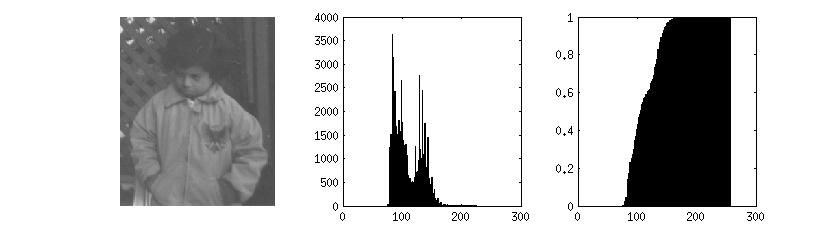
\includegraphics[scale=0.5]{figures/1-3.jpg}
    \caption{Original (left), histogram (middle) and cumulative histogram
    (right)}
    \label{fig:1-3}
\end{figure}

The code used to generate the figure is given in \ref{appendix:histcum}.

% 1.4
\subsection{Floating-point Image CDF}
\begin{multicols}{2}

    The code is given in \ref{appendix:fpimg}.
    
    \vfill{\ }\columnbreak
    
    \begin{figure}[H]
        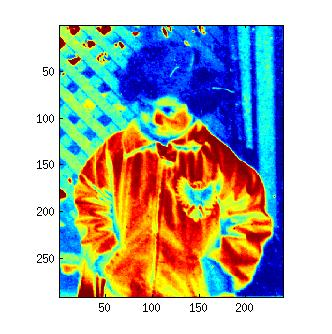
\includegraphics[scale=0.5]{figures/1-4.jpg}
        \caption{Rendition of the floating-point CDF}
        \label{fig:1-4}
    \end{figure}

\end{multicols}

% 1.5
\subsection{Invertibility of CDF}
The CDF is not generally invertible. This is because of the possibly
non-injective characteristics it may present. To overcome this, we may define
a so-called {\it pseudo-inverse} within a given range --- the code for
calculating a pseudo-inverse for a given CDF is shown in
\ref{appendix:pseudo-inverse}.

% 1.6
\subsection{Histogram Matching}
Following equation (3.25) \cite[pp. 74]{SB} we arrive at an equivalent MatLab
function shown in \ref{appendix:histmatch}.

\begin{figure}[H]
    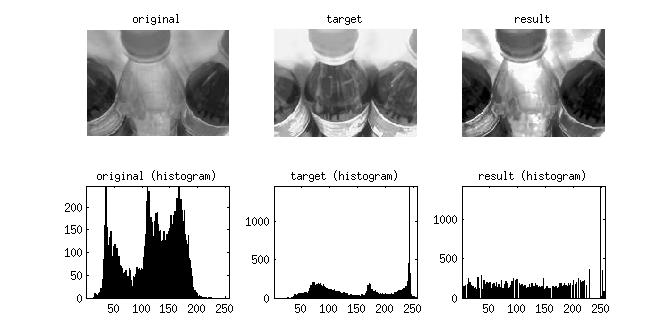
\includegraphics[scale=0.65]{figures/1-6.jpg}
    \caption{Histograms of the matching result}
    \label{fig:1-6}
\end{figure}

% 1.7
\subsection{Matching Algorithm Comparison}
Here we see the results of the previously discussed algorithm, the
implementation of which can be reviewed in \ref{appendix:histmatch}, in
comparison with the built-in MatLab function \code{histeq}.

\begin{figure}[H]
    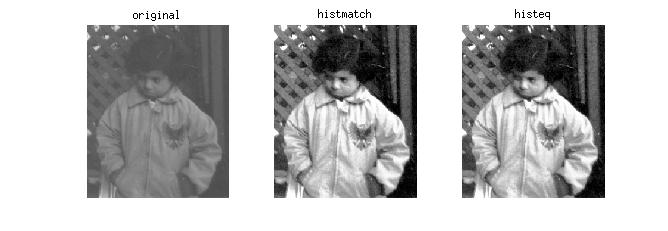
\includegraphics[scale=0.65]{figures/1-7.jpg}
    \caption{Comparison of histogram matching algorithms}
    \label{fig:1-7}
\end{figure}

The program used to generate this figure can be reviewed in \ref{appendix:1-7}

% 1.8
\subsection{Prove the Midway}
I didn't have time to do this one.

% 1.9
\subsection{Simplistic Midway Algorithm}
If we employ the more simplistic mathematical description of the algorithm,
we can generalize it for a sequence of $N$ images. Such an algorithm would
simply calculate the average across all the cumulative histograms in the
sequence.
\begin{align}
    C_m(x) = \frac{1}{N} \sum_{i=0}^{N}C_i(x)
\end{align}

An implementation of the midway specification can be reviewed in
\ref{appendix:midway}.

%
% part2.tex
%

\section{Image Filtering and Enhancement}

\subsection{Finite Difference Approximations}
\begin{align}
    f(x,y) =
    \sum_{i=I_{\text{min}}}^{I_{\text{max}}}
    \sum_{j=J_{\text{min}}}^{J_{\text{max}}}
    w(i,j) \frac{I(i + x + 1, j + y) - I(i + x - 1, j + y)}{2}
    \\
    f(x,y) =
    \sum_{i=I_{\text{min}}}^{I_{\text{max}}}
    \sum_{j=J_{\text{min}}}^{J_{\text{max}}}
    w(i,j) \frac{I(i + x, j + y + 1) - I(i + x, j + y - 1)}{2}
\end{align}

\subsection{Linearly Separable Filters}
These types of filters can be carried out row-by-row, and column-by-column,
since less pixels are affecting the intermediate results, I would think this
is what allows linearly separable filters to be more robust toward noise.

This is a guess, and I didn't have time to put more thought into it than that.

\subsection{Comparison of Mean and Median Filtering}
\begin{multicols}{2}
As we can see from figure \ref{fig:2-3-a} the median filter is much better at
reducing {\it salt and pepper} noise, whilst the mean filter (at least in my
opinion does a somewhat better job at reducing gaussian noise.

The code used to generate the graph on the left, and the image figures below
can be found in the appendix section \ref{appendix:2-3}.
    \vfill{\ }\columnbreak
    
    \begin{figure}[H]
        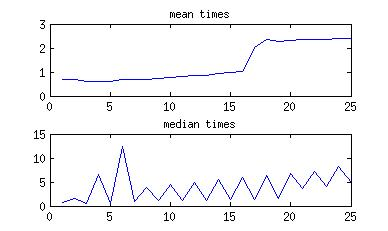
\includegraphics[scale=0.6]{figures/2-3-b.jpg}
        \caption{$x$-axis is $N$ and $y$-axis is number of sec. for 100
        computations}
        \label{fig:2-3-b}
    \end{figure}
\end{multicols}
\begin{figure}[H]
    \center
    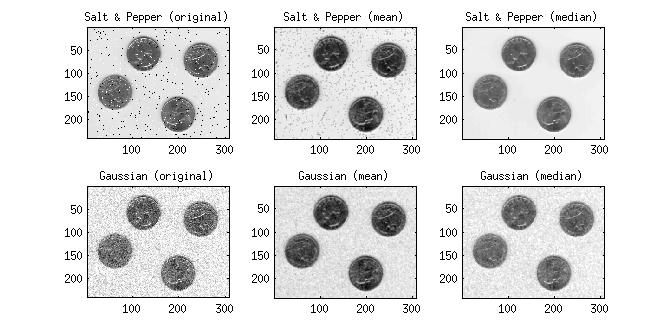
\includegraphics[scale=0.5]{figures/2-3-a.jpg}
    \caption{Showing originals (left), mean filtered (middle) and median
    filtered (right)}
    \label{fig:2-3-a}
\end{figure}

\subsection{Filter Limits}
As we increase $N$ the region affected by the filter gets so large that the
standard deviation $\sigma$ no longer has any effect. In this case, I stop
seeing any differences at approximately $N=15$.

\subsection{Standard Deviation}
Keeping $N > 3\sigma$ we let the filter continue to let the imaginary pixels
outside of the image affect the result, and as we continue to increase
$\sigma$ the image gradually moves towards a single uniform intensity across
the entire image.


% \include{part3}

\appendix
%
% code.tex
%

% usage: \codefig{label}{file}{firstline}{lastline}{description}

\section{Assignments}

\subsection{Cumulative Histogram}
\label{appendix:1-3}
\codefig{1-3}{../assignment1.m}{1}{9}{Cumulative histogram}

\subsection{Floating-point Image CDF}
\label{appendix:1-4}
\codefig{1-4}{../assignment1.m}{11}{17}{Floating-point CDF}

\subsection{Invertibility}
\label{appendix:1-5}
\codefig{1-5}{../assignment1.m}{19}{23}{CDF Invertibility}

\subsection{Histogram Matching}
\label{appendix:1-6}
\codefig{1-6}{../assignment1.m}{25}{37}{Histogram matching}

\subsection{Histogram Matching Comparison}
\label{appendix:1-7}
Notice that we have to supply an image to our custom \code{histmatch}
function --- hence the difference in calculating the arguments. The results
should however both follow the same histogram to match.
\codefig{1-7}{../assignment1.m}{39}{50}{Histogram matching comparison}

\subsection{Simplistic Midway Algorithm}
\label{appendix:1-9}
\codefig{1-9}{../assignment1.m}{52}{65}{Simplistic midway algorithm}

\subsection{Comparison of Filters}
\label{appendix:2-3}

\codefig{2-3}{../assignment2.m}{1}{50}{Filter comparison}

\section{Functions}

\subsection{RGB to Greyscale Conversion Function}
\label{appendix:rgb2grey}
Computing the grey-scale image of an RGB image is done by scaling each channel
using estimated visual perception coefficients\cite[pp. 11]{SB}.
\codefig{rgb2grey}{../rgb2grey.m}{1}{3}{RGB to Greyscale conversion}

\subsection{Cumulative Histogram}
\label{appendix:histcum}
To compute the cumulative histogram we use MatLab's \code{imhist} to calculate
the image histogram, and the cumulative sum thereof, using MatLab's
\code{cumsum}.
\codefig{histcum}{../histcum.m}{1}{4}{MatLab function that computes the
cumulative histogram}

\subsection{Floating-point Image CDF}
\label{appendix:fpimg}
We extract the image data of $I$ interpreting it as floating-point values, or
\code{double}. Then we apply the given \code{cdf} function to each of these
values, returning the result.
\codefig{fpimg}{../fpimg.m}{1}{4}{MatLab function that computes the
floating-point image}

\subsection{Pseudo-inverse of a CDF}
\label{appendix:pseudo-inverse}
We declare a list of the discrete values $\{0,\dots,255\}$ on which $f$ is
defined. For each of these we then apply the \code{cdf} function, and find all
the indices into this list for which the condition $f(s) \geq l$ holds. For
each of these we then apply the previously calculated values. The minimum of
this set is then returned.
\codefig{finv}{../finv.m}{1}{7}{MatLab function that computes a pseudo-inverse
of a given CDF}

\subsection{History-matching}
\label{appendix:histmatch}
On lines 2--3 we calculate $C_x$ and $C_z$, and following that $C_z^{-1}$
based on these on line 4. This results in a CDF that is equivalent to that of
equation (3.25) \cite[pp. 74]{SB}.
\codefig{histmatch}{../histmatch.m}{1}{6}{History matching algorithm}

\subsection{Midway Specification}
\label{appendix:midway}
\codefig{midway}{../midway.m}{1}{3}{Midway specification algorithm}



\begin{thebibliography}{9}

\bibitem{SB}
    Solomon \& Breckon,
    \emph{Fundamentals of Digital Image Processing - A Practical Approach with
    Examples in Matlab},
    2011

\end{thebibliography}

\end{document}

